% LaTeX layout by Jonas Kahler, jonas@derkahler.de
% AutoTux Final Report
% Group Tux:
% Max Enelund, Jerker Ersare, Thorsteinn D. Jörundsson,
% Jonas Kahler, Dennis Karlberg Niklas le Comte, Marco Trifance, Ivo Vryashkov
% Chapter 2 - Algorithmic Aspects
\chapter{Algorithmic Aspects}
%% General stuff by Niklas
\section[General]{General\textsuperscript{[NLC]}}
To create an autonomous miniature vehicle that could complete scenarios such as
lane following, overtaking and parking there had to be a place where these parts
were integrated. That integration point came to be the Decision Maker. The
communication between the Lane Follower and Decision Maker is done using
OpenDaVINCI’s containers and broadcast conferences.

%% Decision Maker by Marco
\section[Decision Maker]{Decision Maker\textsuperscript{[MT]}}
The Decision Maker (DM) is a time-triggered component implementing the car's
state machine and the main logic for controlling the vehicle. Below we list the
states included in the DM state-machine and provide a brief description of their
intended behaviors:\\

\noindent
\textbf{Lane Following}: the vehicle follows the track and stops temporarily
when stop lines are detected. Since control values are exclusively produced by
the Lane Follower, this state assumes a scenario where no obstacles are placed
on the track.\\
\textbf{Driving}: the vehicle follows the lane and overtakes obstacles that are
placed on the track. Control values are produced by the Lane Follower and the
Overtaker object included in the DM.\\
\textbf{Parking}: the vehicle follows the track constantly looking for a parking
spot to perform a parking maneuver. Control values are produced by the Lane
Follower and the Parker object included in the DM. This state assumes a scenario
with no obstacles on the actual lanes.\\
\textbf{Resume}: this state is supposed to resume the car from a parking spot.
It isn't fully developed and tested yet.\\
The current state in the DM state-machine can be switched in the Configurator
Tool.\\

\noindent
To reproduce the behaviors described above, the DM alternates between the
control values shared by the Lane Follower and those produced by the Overtaker
and Parker objects. While the Lane Follower is implemented as time-triggered
component running parallel to the DM, the Overtaker and Parker are two instances
of classes providing control values via public methods that are called by the DM 
according to the current state in its state-machine.\\

\noindent
In addition to selecting and sharing the desired vehicle control values, the DM
is also responsible for:
\begin{itemize}
\item communicating information about which lane the vehicle is currently
   traveling (relevant for overtaking maneuvers in the \textit{driving} state).
\item share light control values.
\end{itemize}

%% Lane Follower by Dennis
\section[Lane Follower]{Lane Follower\textsuperscript{[DK]}}
The responsibility of the Lane Follower component is essentially to process and
compute a desired steering wheel angle based on a picture sent through from the
Proxy component.
The processing and lane detection part is explained in the
\textbf{Algorithm Fundamentals} section. This part will simply explain the
lane-following logic, with the assumption that the image processing and
lane-detection steps are already done.\\

\noindent
\textbf{Lane Following}: The lane-following is based on values extrapolated
during the lane-detection phase. During that phase we measured the distance from
the center of the image to the left and right lines, these distances are
measured in pixels. If the car is completely centered, these values should be
the same. The distance to the lines when the car is perfectly centered is the
value we call ``distance''. The objective of the LaneFollower is to try to keep
both values as close to this distance as possible.\\
When the car is in the right lane, the logic prefers to look at the right line,
only when there are no markings on the right-hand side of the road do we
consider the left line markings. Here we have an example of the algorithm we use
to calculate the desired adjustment:
\begin{center}
\itshape
e - Desired correction\\
x - Distance to right lane marking\\
y - Pixels to the center of the image\\
\vspace{3mm}
e = ((x - y) - distance) / distance
\end{center}
This is what the algorithm looks like when we are following the right line, when
we are following the left line the algorithm looks a bit different, essentially
it is just reversed. It is also worth mentioning that we purposely decided to
offset the entire perception of the image in order to make the car stay more to
the right in the lane. This helps in both parking and overtaking, by keeping to
the right we are closer to the objects considered in the parking and overtaking,
thereby making sure they do not unexpectedly get out of sight. It also improves
the lane-following in sharp right turns where we noticed a recurring behaviour
of the right lane markings getting out of sight for the camera. Altering the
perception of the image seemed like the easiest way to adjust the position of
the vehicle without fiddling with the algorithm.\\
Additionally we also looked into the ideas of  \textit{PID Control}. The
general idea of this control method is to alter the desired correction based on
a few different gains. The one gain we found most useful was the
\textit{Proportional Gain}. The proportional gain is simply multiplied with
the desired correction, if the proportional gain is over 1, desired steering is
increased. If it is below 1, it is decreased. This proved useful when trying to
smooth out the handling in curves. The proportional gain together with the
aforementioned \textit{distance} turned out to be the two values we used to
tweak the LaneFollower for smooth and stable lane-following. The other two gains
\textit{Integral Gain} and \textit{Derivative Gain}, were used when computing
the final desired steering however, we did not attempt to experiment a lot with
these gains seeing as we achieved steady lane-following using only proportional
gain. In the final product we left these very close to 0. The integral gain
would potentially be more useful on a more imperfect track. The derivative gain
could have also been useful if the lane-following played a bigger part in
overtaking maneuvers, but since most of the lane-switching was hardcoded in our
solution, the conditions were already perfect enough when the control was handed
back to the LaneFollower, that we did not have to consider the derivative gain.
For further information about the \textit{PID Control} refer to the Algorithmic
References section.\\

\noindent
\textbf{Overtaking}: The only connection we ended up having in our
implementation between the overtaker and LaneFollower was whether the
LaneFollower should use left- or right-lane handling. This was done by sending a
value from the overtaker to the LaneFollower that simply notified the
LaneFollower if the overtaker had switched lane. Another idea would have been to
have the LaneFollower actively checking if it has passed a lane marking and
using that as an indication whether the car is in the right or left lane.
However, we ended up using the first method since we figured that the only point
at which the car actually switches to the left lane is when it is overtaking,
making the first solution seem more appropriate in our implementation. In our
solution though, the overtaker completely takes over during the duration of the
lane switches, making any other information except which lane we were in
unnecessary for the LaneFollower.\\

\noindent
\textbf{Speed limitations}: Even during pure lanefollowing with no other
algorithm such as overtaking or parking running, the speed of the car in our
current implementation is quite limited. Due to limited testing time and other
components such as the parker and overtaker needing to be tested thoroughly, we
did not budget our time well enough to properly optimize the LaneFollower at
higher speeds. We ended up opting for a slower speed with a smoother ride,
seeing as we needed to drive at a slower speed to properly test the other
components. We found that one of the main problems with traveling at a higher
speed could have been the time it took for the data to travel through the
components. The time it took for the camera to capture the image, the Proxy
forwarding it to the LaneFollower  and the LaneFollower suggesting a steering
angle, was too long for it to be accurate by the time it reached low-level board
when driving at higher speeds. Looking back at it now, one simple solution that
might have solved that for us could have been to simply move the point at which
we do the detection a bit further ahead. It would require a bit of testing but
we are quite certain that by applying this change, we could have found a happy
medium for a higher speed.

% Overtaking by Marco
\section[Overtaking]{Overtaking\textsuperscript{[MT]}}
The logic for overtaking maneuvers is implemented in the Overtaker class. The
basic idea behind the overtaker is that it should constantly perform some
\textit{obstacle detection} operations while the car is controlled by the
LaneFollower. Whenever an overtaking maneuver is initiated, the overtaker takes
control of the vehicle to perform the necessary maneuvers and, once these are
completed, it releases the control back to the LaneFollower.\\
The overtaker contains its own state-machine and uses sensors and wheel encoder
values to handle transitions between states. The sensors that are relevant for
the overtaker are the front-forward and front-right ultrasonic sensors as well
as the front-right and the rear-right infrared sensors.\\
Figure~\ref{otfsma} below displays the overtaker state-machine and indicates the
operations that are executed in each state and the conditions that trigger
transitions. Operations performed in each state are labeled as the functions
implemented in the Overtaker.cpp module (for the sake of readability we decided
to omit the function parameters). Orange boxes denote states where the overtaker
controls the vehicle directly, while blue boxes indicate states where the
overtaker activity is limited to understanding the surroundings and checking the
conditions that trigger the transition to the next state.
\begin{figure}[ht]
  \centering
  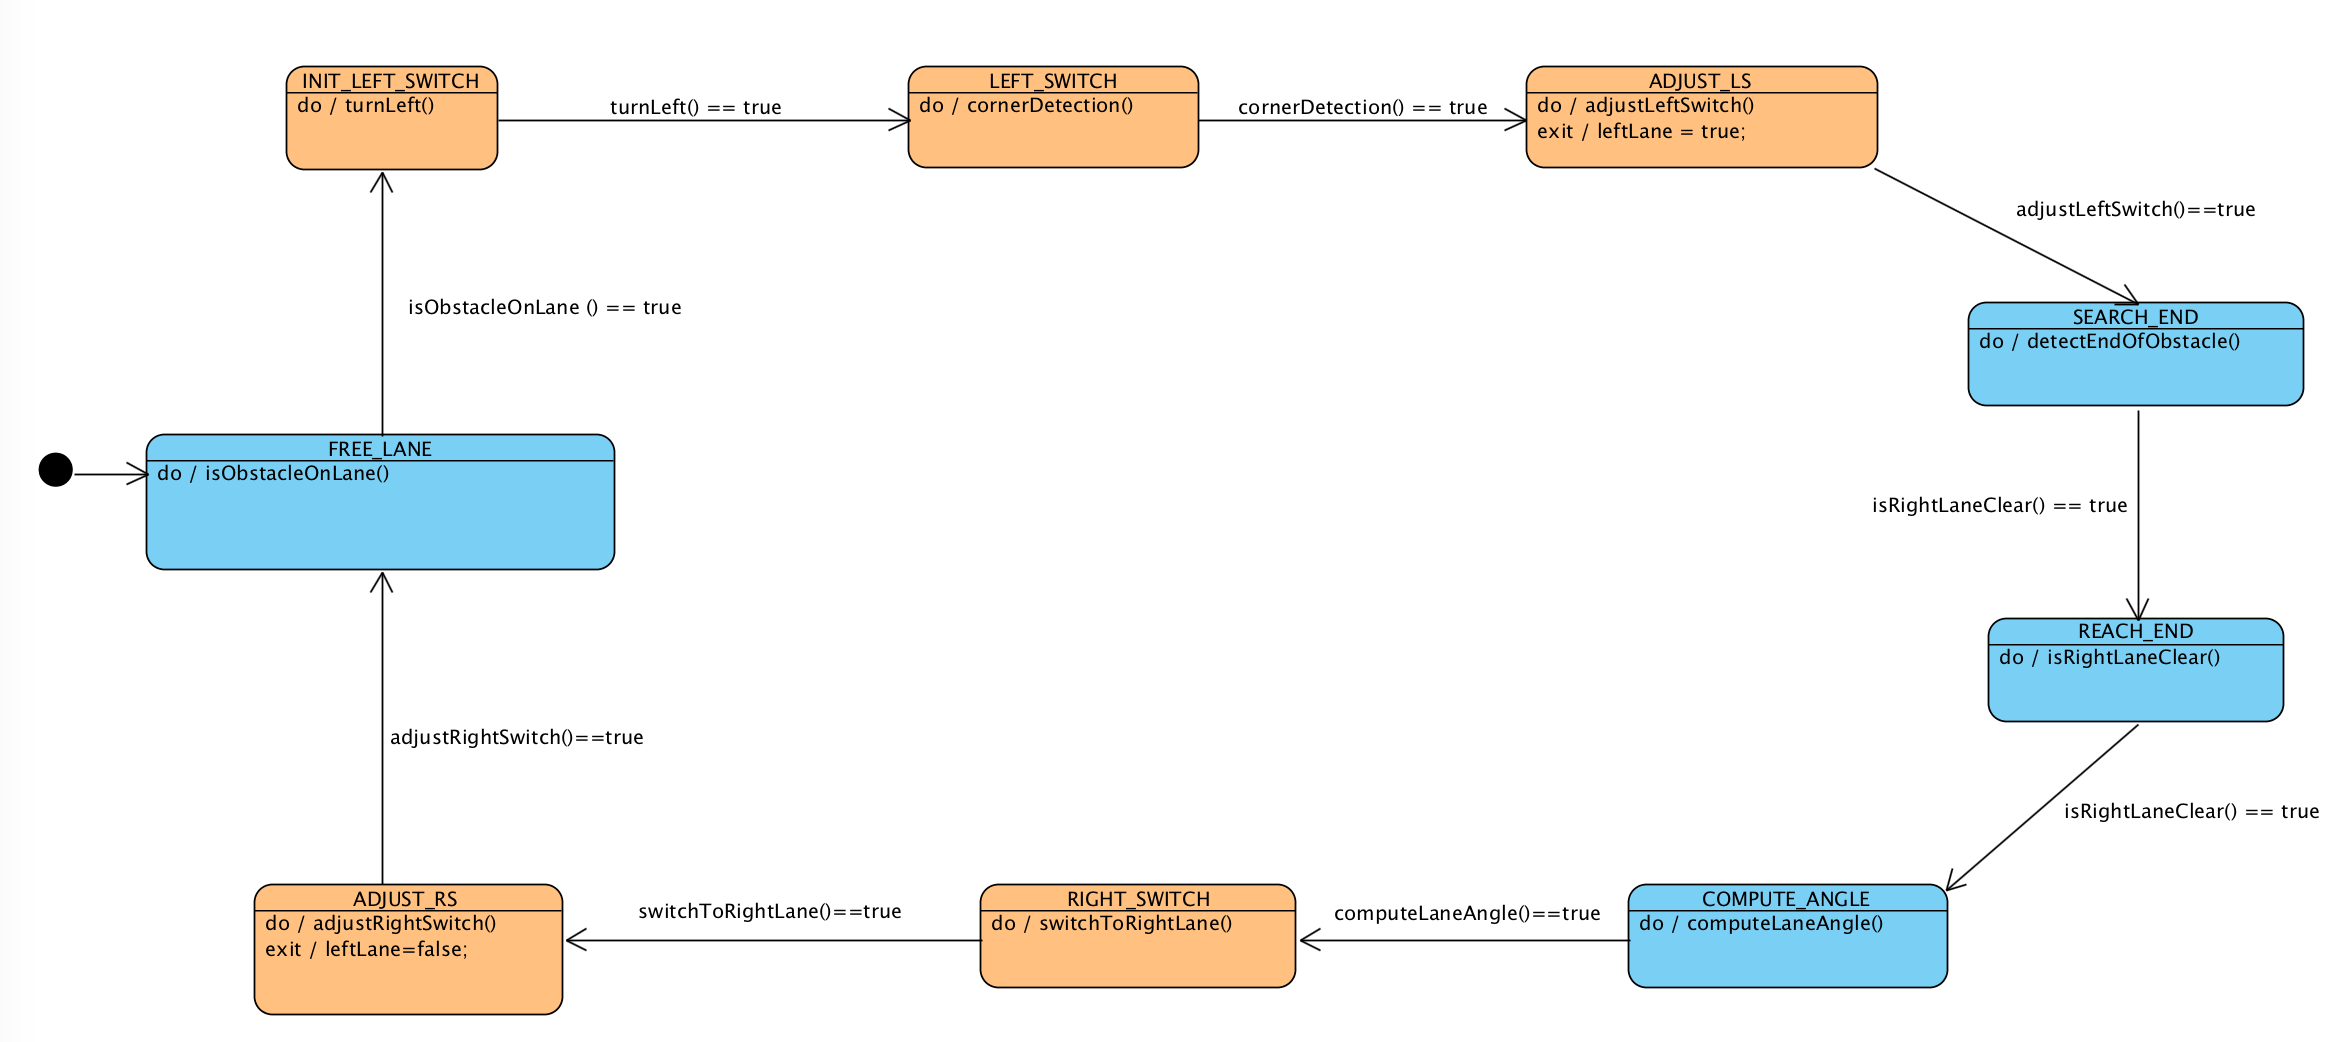
\includegraphics[width=1\textwidth]{160515_Overtaker_FSM.png}
  \caption{Overtaker FSM}
  \label{otfsma}
\end{figure}
Below we provide a brief description of the operations performed in each state
together with the conditions that trigger transitions from a state to another.\\

\noindent
\textbf{Free-Lane}: we use the front-center ultrasonic sensor to look for
obstacles to overtake. If an obstacle is detected within a distance below a
fixed threshold (7.0 in the simulator), the overtaker takes control of the car
and transitions to \textit{Init Left Switch}.\\

\noindent
\textbf{Init Left Switch}: the vehicle steers left 30\degree and travels a path
of fixed length (3.0 in the simulator) before moving on to the next state. The
reason why we introduced this state is simply to move the car enough to make the
front-right ultrasonic sensor point at the back of the obstacle that is being
overtaken so that the corner detection algorithm can be performed correctly in
the following state. We are aware that this state could lead to undesired
behavior, especially if the length of the path is not estimated correctly. More
in details, by using this algorithm we are ``hoping'' that the front-right
sensor is pointing at the obstacle when the state machine transitions to the
next state. A viable and probably more solid option would be that of using the
gyro sensor to determine the target heading that will point the front-right
ultrasonic sensor at the obstacle. Due to time constraints, we could not
implement this logic before the final presentation, and therefore we opted for
this quick fix instead.\\

\noindent
\textbf{Left Switch}: the vehicle keeps steering left while using the
front-right ultrasonic sensor to detect when the car has passed by the rear-left
corner of the obstacle. Once the corner is detected, the FSM transitions to the
next state.\\

\noindent
\textbf{Adjust Left Switch}: this state is responsible for completing the
left-switch maneuver by steering right approximately 12\degree and traveling for
a fixed-length path (3.6 in the simulator). The rationale behind this state is
to move the vehicle in a position that is likely to improve the camera's ability
understand the lane and produce the desired steering control values in the next
state. After the adjustment maneuver is completed, the overtaker sets the
current lane to \textit{left} and releases the control back to the LaneFollower.
\\

\noindent
\textbf{Search End}: at this point the vehicle is controlled by the LaneFollower
instructions. This allows the vehicle to correctly follow the lane while
overtaking on curves. Our implementation of the Lane Follower  aims to keep the
car closer to right side of the lane when traveling on the left lane. By doing
so, we ensure the right side infrared sensors not to lose sight of the obstacle
that is being overtaken, therefore allowing the overtaker to detect the end of
the obstacle. As soon as the front-right ultrasonic sensor stops detecting the
obstacle while the infrared sensors still detect it, the state-machine
transitions to the next state.\\

\noindent
\textbf{Reach End}: the overtaker uses the right side sensors to determine when
the vehicle has reached the end of obstacle. When all three right side sensors
(ultrasonic front-right and infrared front-right and rear-right) stop detecting
the obstacle, the overtaker FSM moves on to the \textit{Compute Angle} state.\\

\noindent
\textbf{Compute Angle}: this state is responsible for detecting curves on the
area of the track where the vehicle is going to perform the switch to the right
lane. We do so by computing an average of the recommended steering angle from
the LaneFollower over 5 frames and by comparing this value with some fixed
thresholds (below -0.13 radians for a left turn, above 0.1 for a right turn).
This estimation allows us to adjust the values of the desired steering angle and
the length of the path to travel depending on whether the right switch maneuver
will be performed on a left turn, right turn or on a  straight lane.\\

\noindent
\textbf{Right Switch}: during the right-switch the vehicle steers right and
travels over a fixed-length path before transitioning to the next state. The
values for steering angle and path length are set accordingly to the results
from the computations performed in the previous state.\\

\noindent
\textbf{Adjust Right Switch}: this state is responsible for adjusting the car on
the lane before to return the vehicle controls to the LaneFollower. We do so by
steering left approximately 30\degree and travel for a fixed-length path (2.0 in
the simulator). Once the vehicle has traveled enough, the overtaker releases the
control of the vehicle, updates information on the current lane and transitions
to the initial state \textit{Free-Lane}.\\

\noindent
In order to avoid transitions to be triggered by noise in sensors values, we
require the conditions that are based on sensor values to hold for 3 consecutive
frames before transitioning to next state. However, it is worth saying that
sensor readings used by the overtaker are already smoothed via moving averages
as explained later in the Environment Detection section on.\\

\noindent
Figure~\ref{otfsmb} displays the values returned by the sensors during an
execution of an overtaking maneuver run in the simulator. The recording for this
simulation are provided in file overtaking\textunderscore noise.rec that was
submitted together with this document. The horizontal black dotted line denotes
the threshold used by the ultrasonic front-forward sensor to trigger the
transition from \textit{Free-Lane} to \textit{Init Left-Switch}. Thus, the
transitions described above take place in the area of the diagram to the right
of the intersection between the black dotted line and the orange line. The init
left-switch state moves the car in a position that allows the front-right
ultrasonic sensor to ``see'' the obstacle (red line) so that corner detection
can be performed in the left-switch state. The switch between left switch and
adjust left-switch takes place immediately after the local minimum displayed by
the red line, which represents the distance between the front-right us sensor
and the rear-right corner of the obstacle. The following readings display the
states adjust left-switch and search-end. The transition from search-end to
reach-end is triggered as soon as the red line signals -1, while reach-end to
compute-angle is triggered as soon as the rear-right infrared sensor (green
line) reads -1. The final two states right switch and adjust right switch only
use the wheel encoder and therefore cannot be described in terms of sensors
values.
\begin{figure}[ht]
  \centering
  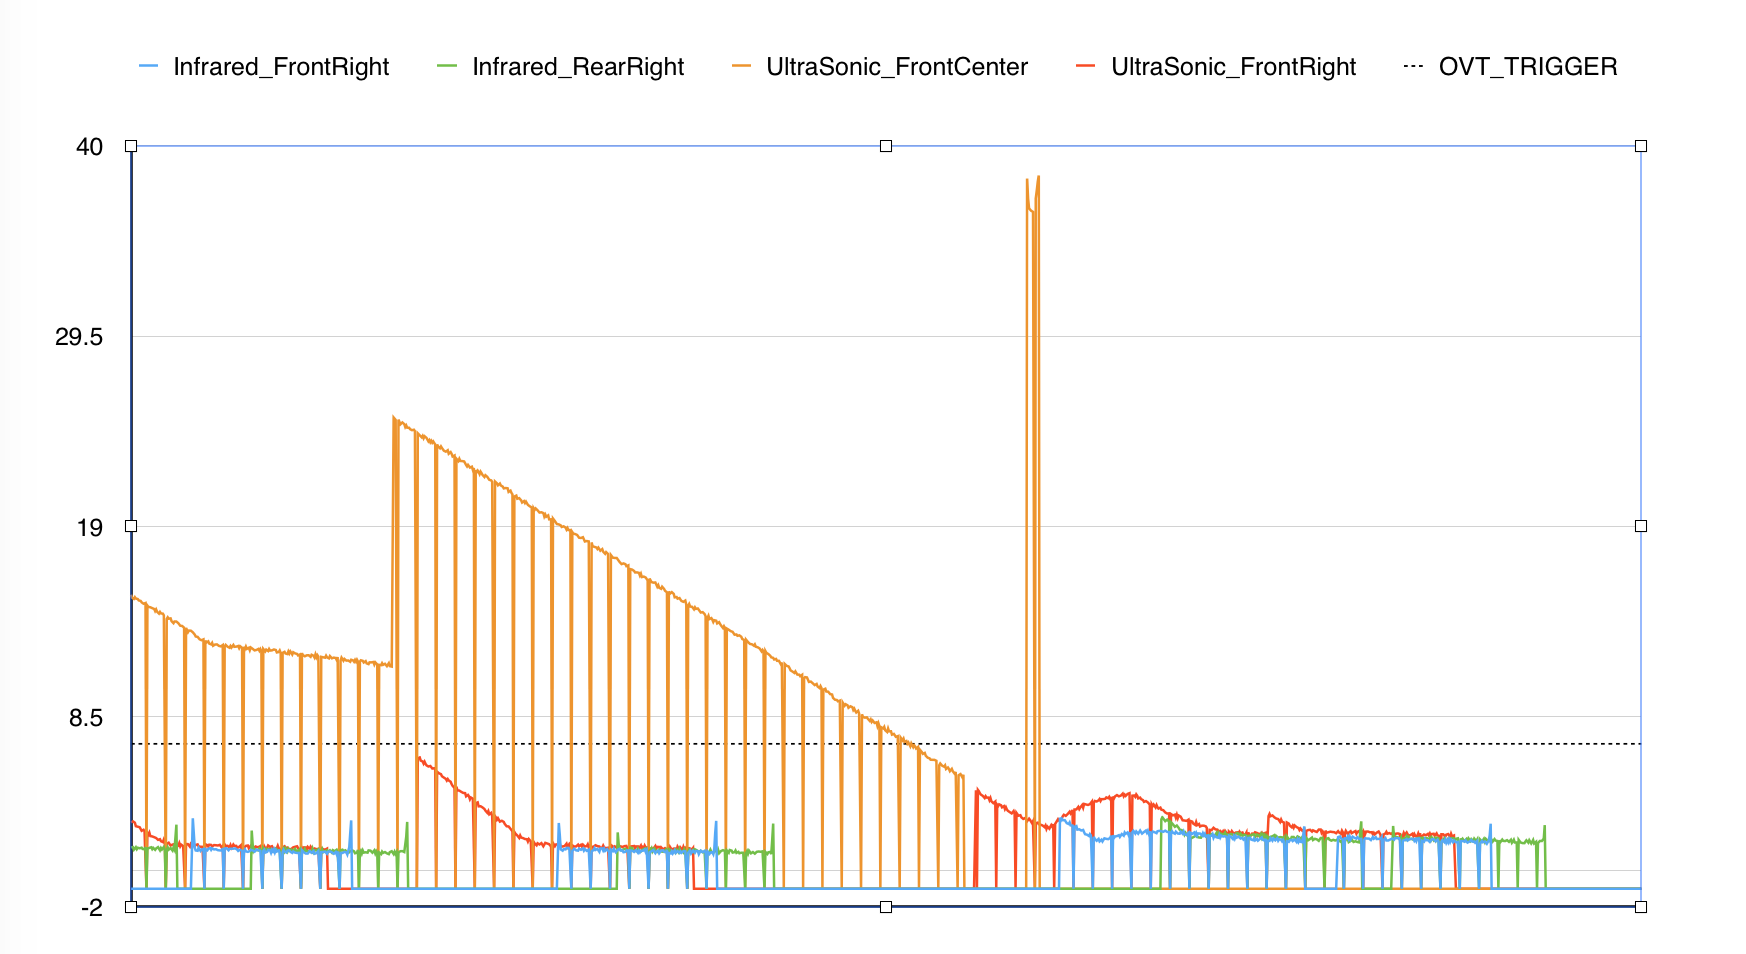
\includegraphics[width=1\textwidth]{160516_Overtaker_FSM.png}
  \caption{Overtaker FSM}
  \label{otfsmb}
\end{figure}
The logic described above is based on some assumptions that work perfectly in
the simulator environment but might generate wrong behavior if applied to a
real-world scenario. For example, the \textit{corner detection} algorithm
requires some sort of regularity in the shape of the obstacle. Irregularities
such as a non-flat rear surface are likely to lead to a wrong detection of the
corner and finally have the car to initiate the adjust maneuver too early or too
late. Another assumption is that obstacles should never be positioned in a way
that makes them trespass the broken line that separates the two lanes. If we
were to test the overtaker in a scenario that does not meet this requirement, we
would probably see the vehicle collide with the obstacle during the Search-End
or Reach-End state. This is due to the fact that the LaneFollower is controlling
the car during those states, while the overtaker is using the sensors only to
detect the end of the obstacle. Introducing adjusting maneuvers based on sensor
values would definitely allow to relax this assumption, but at the cost of
compromising the estimations performed during the \textit{Compute Angle} state.

%% Parking by Niklas
\section[Parking]{Parking\textsuperscript{[NLC]}}
To realize a parallel parking scenario for an autonomous miniature vehicle there
had to be a state machine. The implementation of the logic is inside the Parking
class and the final state machine can be viewed below. It consists of five
different identified states; searching, measuring, parking, parked and resume.
The two states searching and parking both consists of sub-states. The Parking
has public methods which the DM is using to know where in the parking it is,
e.g. has found a parking spot, or if it is reversing or not (for the lights on
the car). The reasoning about the parallel parking was that the car should
always be able to park within a certain amount of distance between two objects.
From that it should never fail the parking. Also to make it parallel inside the
spot it has to travel roughly the same distance with each steering wheel angle
to get it straight inside the parking spot. With this understanding the parking
scenario was created as written below.
\begin{figure}[ht]
  \centering
  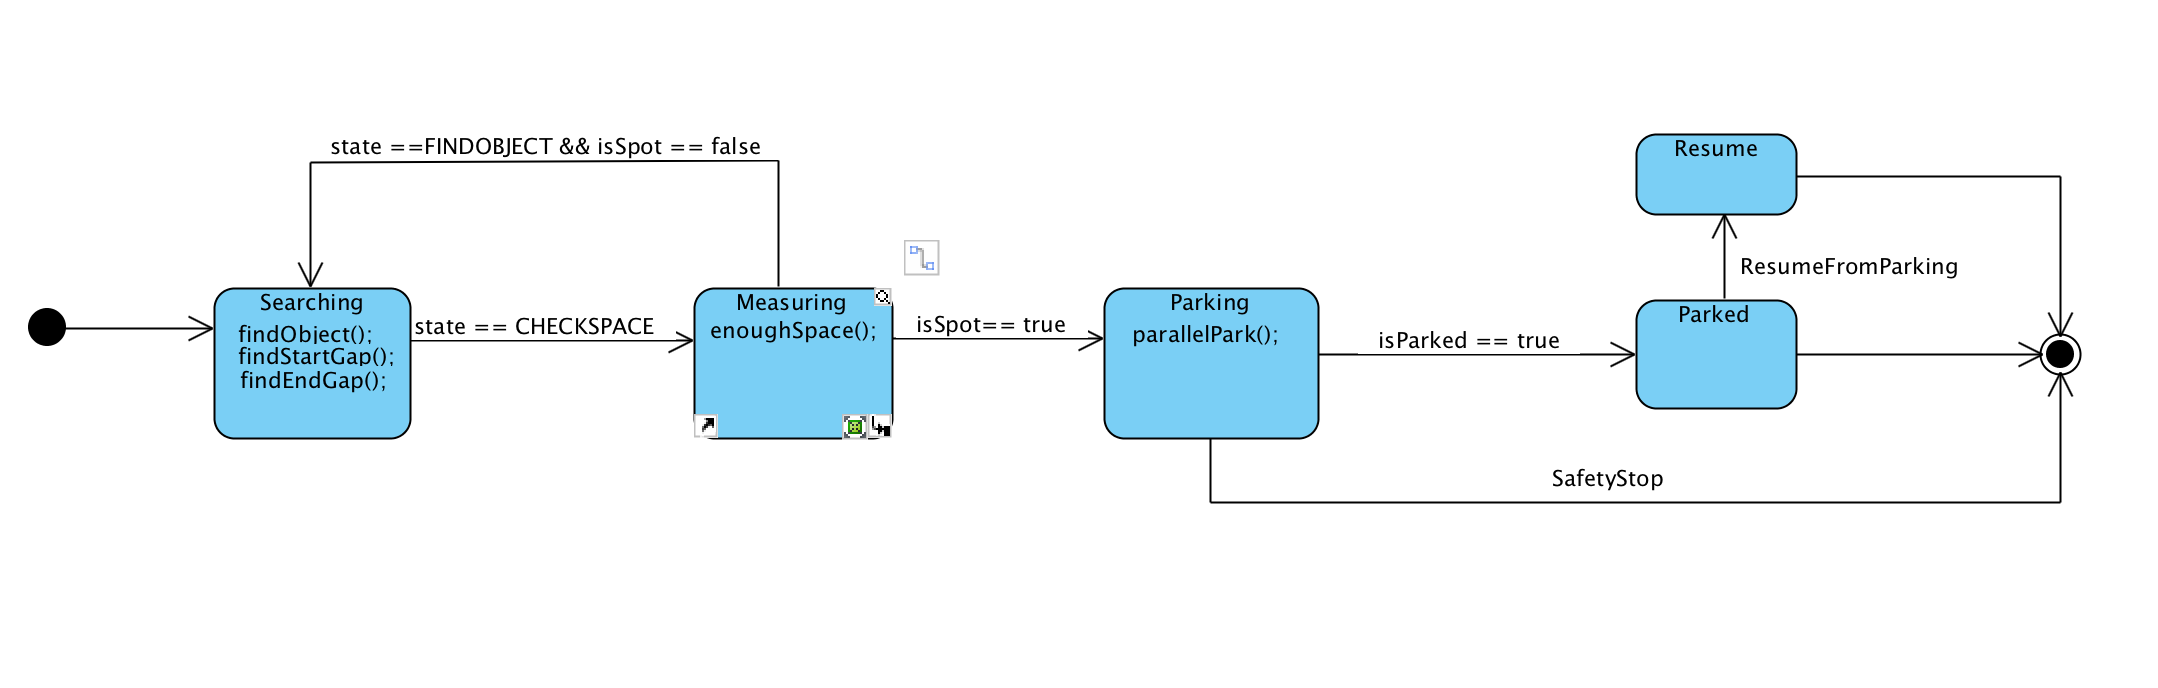
\includegraphics[width=1\textwidth]{ParkingScenarioSTM.png}
  \caption{Parking FSM}
  \label{otfsmb}
\end{figure}
To handle the noise data for both the simulation and from the real world there
is a counter implemented that checks that there isn't any off data from the
sensors making any state changes within the logic. This changed on some parts of
the code later in the project due to always getting average values from the STM,
and the code was more focused on the real car instead of the simulation (which
gave noise data on every sensor at the same time).\\

\noindent
\textbf{Searching}: To be able to judge if there exists a place for the car to
park it needs to make use of at least one or two sensors. This parking is using
the rear right infrared sensor and the wheel encoder for the detection of a
parking spot. The rear right infrared sensor was chosen because then the car
will end up in a good start position with only a small adjustment. The wheel
encoder plays a huge part for the parking scenario, with its help it is possible
to measure lengths, e.g. the size of a gap. During the searching state the car
should still be controlled by the LaneFollower for staying in a good position on
the track and keep the car on the lane, and when a spot has been found the
parking will take over in DM. To determine if an object are detected by the
sensors is that the values from the sensors will decrease, and the opposite goes
for not seeing anything (in OpenDaVINCI simulation seeing nothing is -1 from the
sensors). With that understanding it is possible to detect an object and when it
ends. From when a gap is detected (end of an object) the current traveled
distance can be stored for measuring the size of the gap. The next step is to
find if there is another object coming up ahead or that the distance from the
back object is long enough for the car to park (only if the car hasn't been
inside a curve where it in that case makes it go back to the first state). This
can be done by the same logic as for detecting the first object and then stores
the current traveled distance from where the gap ends. This felt like the most
reliable way of detecting gaps between object.\\

\noindent
\textbf{Measuring}: This state's purpose is to check if the gap is big enough to
park in. The stored value for the end of the gap minus the stored value for the
beginning of the gap will give the size of the gap. This size can then be used
to compare if the size is bigger than a limit set for what the car can park
inside. If it isn't big enough it transitions back to the searching state,
otherwise it continues to the parking state.\\

\noindent
\textbf{Parking}: Within this state the parking routine is executed. Every step
of these sub-states returns vehicle control data for the DM to control the car.
The parking state is making use of the ultrasonic front sensor, the infrared
rear back sensor and the wheel encoder to execute the parallel parking maneuver.
The ultrasonic sensor is relevant because there will be an object in front of
the car and the car should not hit it, the same reasoning goes for the infrared
sensor but for the back object. The wheel encoder is used to determine how much
the car has traveled inside of the sub-states, so that it is possible to get the
car straight inside the parking spot as mentioned above. The distance is used
for the state switching inside the different states. The sub-states are:
\textit{phase0, phase1, phase2, phase3, phase4} and \textit{safety stop}.\\

\noindent
\textbf{Phase0}: This sub-state's goal is to take the car into a good position
before starting the parking. This is important because to be able to get into
the parking spot with a good angle while reversing it has to get into a good
position to the front object.\\
\textbf{Phase1}: This sub-state's goal is to reverse around the back left corner
of the front object. The car will turn the wheel angle 0.5 radians and reverse
the set amount of distance. It will then get a good angle to get into the
parking spot.\\
\textbf{Phase2}: This sub-state's goal is to reverse straight back into the spot
to adjust the depth of the parking. This is mainly used inside the OpenDaVINCI
simulation due to that the car is a further out and to get it into the middle of
the spot in a nice position it has to back straight for a bit. It was not needed
on the real car because the objects were next to the road and it got into a nice
position with only \textit{phase1} and \textit{phase3}.\\
\textbf{Phase3}: This sub-state's goal is to get parallel inside the parking
spot. It starts turning the wheel angle to -0.5 radians while it is reversing.
As stated above the car is using the wheel encoder for the distance to know when
it has straighten up inside the parking spot. It is in this state it's making
the most use of the ultrasonic front sensor and the infrared rear back sensor.
It is using them to not hit any of the objects it is parking in between and also
be able to park within smaller spaces. When it get’s too close to the back
object it is switching to go forward instead with the wheel angle 0.5 radians.
If it hasn't finished the distance yet and gets too close to the front object
it's starts reversing again with -0.5 radians. All this is repeated until the
car has traveled the set distance to get parallel. One problem we discovered
within this state was that for the real car there is a delay with the sensor
readings. It reacted on the different triggers too late so that the car collided
with the objects. To fix this we increased the threshold to be longer and it had
more time to process the information, that fixed the issue but could have made
it so that it can't get into a certain size of gaps.\\
\textbf{Phase4}: This sub-state's goal is to get into the middle of the parking
spot with good distance from the back and front objects. It is still depending
on the front ultrasonic sensor and the infrared rear sensor and here the wheel
encoder isn't used anymore for the parking. It has only the wheel angle 0
radians set. This state has two different paths to go depending on if there was
an object in the front or not, but they are similar in their functionality. They
are checking which of the sensor readings is the bigger one and then adjust the
position based on that. To know if it is inside the middle of the parking spot
there is a comparison between the sensors and an acceptance range that the
difference should be less than.\\
\textbf{Safety stop}: This sub-state's goal is to stop the car if there is an
object to close to the car. This is a safety mechanism that should make the car
not to drive into objects when objects are too close to the car. It is not
active when the car itself is inside the parking spot because it is already
using the sensors to switch directions.\\

\noindent
\textbf{Parked}: This state is when the car is done with the parking. The
parking routine is completed and won't do anything anymore. This state is
connected to the DM via a public function that returns a boolean for if the car
is parked. The state has traveled into a do nothing state within the DM and it's
waiting for a new input (resume) or to turn it off.\\

\noindent
\textbf{Resume}: This state is for taking the car out from the parking spot and
then continue to the lane following. This was only an extra feature to make the
car be more as in the real world where it can continue to drive even if it has
been parked.
\begin{figure}[ht]
  \centering
  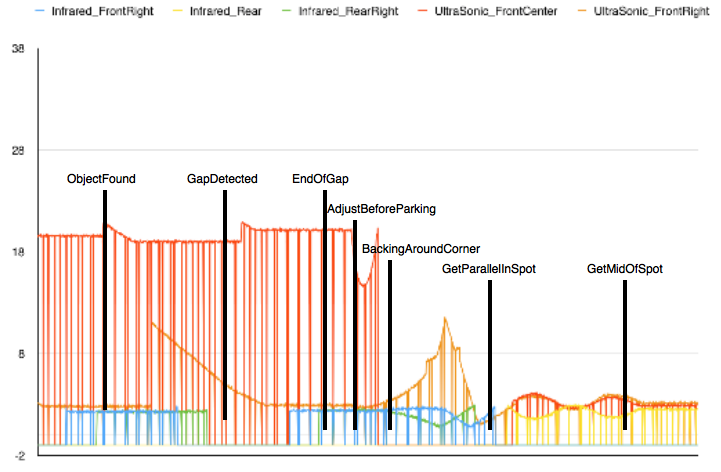
\includegraphics[width=1\textwidth]{ParkingScenario.png}
  \caption{Every stage in the parking can be seen in the sensor value diagram.}
  \label{otfsmb}
\end{figure}
We don't know how the realization of the parallel parking could have been done
in a different way that we made it. The only thing that comes to mind is to have
used the Gyro instead of the distances inside the spot in phase3 to make it to
be parallel inside the parking spot. The Gyro wasn't connected because we felt
that using the distances was good enough to use for completing the task.